
\let\negmedspace\undefined
\let\negthickspace\undefined
\documentclass[article]{IEEEtran}
\usepackage[a5paper, margin=10mm, onecolumn]{geometry}
%\usepackage{lmodern} % Ensure lmodern is loaded for pdflatex
\usepackage{tfrupee} % Include tfrupee package

\setlength{\headheight}{1cm} % Set the height of the header box
\setlength{\headsep}{0mm}     % Set the distance between the header box and the top of the text

\usepackage{gvv-book}
\usepackage{gvv}
\usepackage{cite}
\usepackage{amsmath,amssymb,amsfonts,amsthm}
\usepackage{algorithmic}
\usepackage{graphicx}
\usepackage{textcomp}
\usepackage{xcolor}
\usepackage{txfonts}
\usepackage{listings}
\usepackage{enumitem}
\usepackage{mathtools}
\usepackage{gensymb}
\usepackage{comment}
\usepackage[breaklinks=true]{hyperref}
\usepackage{tkz-euclide} 
\usepackage{listings}                                       
\def\inputGnumericTable{}                                 
\usepackage[latin1]{inputenc}                                
\usepackage{color}                                            
\usepackage{array}                                            
\usepackage{longtable}                                       
\usepackage{calc}                                             
\usepackage{multirow}                                         
\usepackage{hhline}                                           
\usepackage{ifthen}                                           
\usepackage{lscape}

\renewcommand{\thefigure}{\theenumi}
\renewcommand{\thetable}{\theenumi}
\setlength{\intextsep}{10pt} % Space between text and floats

\numberwithin{figure}{enumi}
\renewcommand{\thetable}{\theenumi}

% Marks the beginning of the document
\begin{document}
\bibliographystyle{IEEEtran}
\title{NCERT-9.4.5}
\author{EE24BTECH11035 - K TEJA VARDHAN}
{\let\newpage\relax\maketitle}

\noindent\textbf{Question: }  
Find the solution of the differential equation:  
\begin{align}
(e^x + e^{-x}) \, dy = (e^x - e^{-x}) \, dx
\end{align}

\noindent\textbf{Solution:}  
Rewriting the equation:  
\begin{align}
    (e^x + e^{-x}) \, dy = (e^x - e^{-x}) \, dx
\end{align}

\noindent Let:

\begin{align}
    v = e^x + e^{-x}
\end{align}


\noindent Differentiating $v$ with respect to $x$:  
\begin{align}
    \frac{dv}{dx} = e^x - e^{-x}
\end{align}

\noindent Thus:  
\begin{align}
    e^x - e^{-x} = \sqrt{v^2 - 4}
\end{align}

\noindent The given equation becomes:
\begin{align}
    v \, dy = \sqrt{v^2 - 4} \, dx
\end{align}

\noindent   Substitute:
\begin{align}
    dx = \frac{dv}{\sqrt{v^2 - 4}}
\end{align}

\noindent   This leads to:
\begin{align}
   v \, dy = dv
\end{align}

\noindent  Rewrite:
\begin{align}
   dy = \frac{1}{v}, dv
\end{align}

\noindent  Integrate both sides:
\begin{align}
   \int dy = \int \frac{1}{v} \, dv
\end{align}

\begin{align}
   y = \ln|v| + C
\end{align}

\noindent Substitute $v = e^x + e^{-x}$ back:
\begin{align}
   y = \ln(e^x + e^{-x}) + C
\end{align}

\noindent The solution to the differential equation is:

\begin{align}
  \boxed{y = \ln(e^x + e^{-x}) + C}
\end{align}



where $C$ is the constant of integration(Here, it is assumed as 0).

\vspace{0.5em}

\noindent\textbf{Numerical Approach:}\\ I used a for loop for finding the $y$ values as the loop proceeds with iterative formula given below. I took some initial value of $x$ and as loop proceeds I assigned it the value as $x+h$. where $h$ is the step size, representing the rate of change. 
\\2. Assigned the values of $y$ for different $x$-values using a for loop.  

\noindent The iterative formula for updating $y$-values is:  
\begin{align}
    y_n = y_{n-1} + \left(\frac{dy}{dx}\right) h,
\end{align}
The iterative formula for updating $x$-values is: 
\begin{align}
    x_n=x_{n-1}+h
\end{align} 

\noindent\textbf{Initial Conditions:}  
\begin{itemize}
    \item $x = 0$  
    \item $y = \ln2$  
    \item $h = 0.01$  
\end{itemize}

Using Matplotlib, I plotted the computed points and the graph of the exact solution to verify that they approximately match.
\begin{figure}[h!]
	\centering
	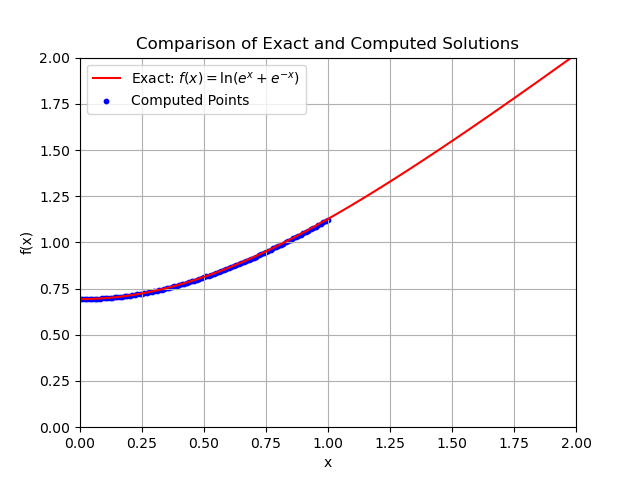
\includegraphics[width=0.5\textwidth]{/home/teja-vardhan/scientific_computing/problem1/figs/p1.png}
	\caption{verifying through graph of sim and theory values}
	\label{stemplot}
\end{figure}	
\end{document}
